\chapter{剪切自锁问题}
本章针对中厚板的剪切自锁问题,提出免剪切自锁的有限元无网格混合离散方案。首先,基于中厚板的本构特性,分析了传统有限元分析过程中产生剪切自锁现象的原因。基于LBB稳定系数误差估计和多项式空间,确定剪切自锁问题的最优约束比取值范围。随后,确定剪切自锁问题的有限元无网格混合离散方案,并通过典型弹性力学算例验证其正确性。
\section{中厚板问题}    
考虑如图\ref{ch_5:fig:mindlin_picture}所示中厚板,板厚为$h$,$\Omega$为板中面。在Mindlin假设下,中厚板考虑横向剪切变形,相应的控制方程由下式给出:
\begin{equation}\label{ch_5:eq:strong_mindlin}
    \begin{cases}
        M_{\alpha\beta,\beta} - Q_\alpha = 0 & \textrm{in}\; \Omega \\
        Q_{\alpha,\alpha} + \bar q = 0 & \textrm{in}\; \Omega \\    Q_\alpha n_\alpha = \bar Q & \textrm{on}\; \Gamma_Q \\
        M_{\alpha\beta} n_\beta = \bar M_\alpha & \textrm{on}\; \Gamma_M \\
        \varphi_\alpha = \bar \varphi_\alpha & \textrm{on}\; \Gamma_\varphi \\
        w = \bar w & \textrm{on}\; \Gamma_w \\
    \end{cases}
\end{equation}
\begin{figure}[!h]
    \centering 
        \includegraphics[scale=0.4]{figures/ch_5/Mindlinplate.png}
        \caption{中厚板运动学及边界条件}\label{ch_5:fig:mindlin_picture}
\end{figure}
式中,$M_{\alpha \beta}$ 可表示弯矩张量$ \boldsymbol{M}$ 的弯曲或扭转部分的分量,$Q_\alpha$为剪力张量$\boldsymbol{Q}$的分量,$\bar{q}$ 为垂直于板中面的分布荷载;
$\Gamma_w$和$\Gamma_\varphi$为本质边界条件,$\bar{w}$和$\bar{\varphi}_\alpha$分别为本质边界条件上给定的挠度和转角;
$\Gamma_Q$ 和$\Gamma_M$ 为自然边界条件,$\bar Q$和$\bar{M}_{\alpha}$ 为自然边界上的等效剪力和法向弯矩;
$n_\alpha$为边界上外法线方向$\pmb{n}$的分量。

在平面应力假设下,对于各同向性线弹性材料,其本构关系表示为:
\begin{equation}\label{ch_5:eq:mindlin_M}
    M_{\alpha \beta}=-\frac{h^3}{12}D_{\alpha \beta \gamma\eta}\kappa_{\gamma\eta}=\frac{h^3}{12}D_{\alpha \beta \gamma\eta}\varphi_{\gamma,\eta}
\end{equation}
\begin{equation}\label{ch_5:eq:mindlin_Q}
    Q_{\alpha}=k\frac{Eh}{2(1+\nu)}\gamma_\beta=kGh(-\varphi_\beta+w_{,\beta})
\end{equation}
其中,$k$为剪切修正系数,$\kappa_{\alpha\beta}$为曲率张量$\pmb\kappa$的分量,$\gamma_\alpha$为剪切应变矢量$\pmb\gamma$的分量,表达式为:
\begin{equation} \label{ch_5:eq:kappa}
    \kappa_{\alpha\beta}=-\varphi_{\alpha,\beta},\quad\gamma_\alpha=-\varphi_\alpha+w_{,\alpha}
\end{equation}
式中$D_{\alpha \beta \gamma\eta}$为在平面应力假设下四阶弹性张量的分量,表达式为:
\begin{equation} 
    D_{\alpha \beta \gamma\eta}=\frac{E}{1-\nu^2}(\nu\delta_{\alpha\beta}\delta_{\gamma\eta}+\frac{1}{2}(1-\nu)(\delta_{\alpha\gamma}\delta_{\beta\eta}+\delta_{\alpha\eta}\delta_{\beta\gamma}))
\end{equation}

根据最小势能原理,强形式\eqref{ch_5:eq:strong_mindlin}所对应的势能泛函表达式为: 
\begin{equation}\label{ch_5:eq:potential_energy}
    \begin{split} 
        \Pi(w,\boldsymbol{\varphi})&=\frac{1}{2}\int_{\Omega}\kappa_{\alpha\beta}M_{\alpha\beta}d\Omega+\frac{1}{2}\int_{\Omega}\gamma_{\alpha}Q_{\alpha}d\Omega\\
        &+\int_{\Gamma_{M}}\varphi_{\alpha}{\bar{M}_{\alpha}}d\Gamma-\int_{\Gamma_{Q}}{w}\bar {Q}d\Gamma-\int_{\Omega} w\bar{q}d\Omega
    \end{split}
\end{equation}
对式\eqref{ch_5:eq:potential_energy}进行变分可得伽辽金弱形式:
\begin{equation}\label{ch_5:eq:weak_penalty_mindlin}
    \begin{split} 
        \text{Find}\,&(w,\varphi_{\alpha})\in V\\
        &\int_{\Omega}\delta\kappa_{\alpha\beta}M_{\alpha\beta}d\Omega+\int_{\Omega}\delta\gamma_{\alpha}Q_{\alpha}d\Omega=\\
        &-\int_{\Gamma_{M}}\delta\varphi_{\alpha}{\bar{M}_{\alpha}}d\Gamma+\int_{\Gamma_{Q}}{\delta{w}}\bar {Q}d\Gamma+\int_{\Omega} \delta{w}\bar{q}d\Omega,\quad \forall(\delta w,\delta\varphi_{\alpha}) \in V
    \end{split}
\end{equation}

对于考虑横向剪切变形的中厚板,根据中厚板的本构关系\eqref{ch_5:eq:mindlin_M},\eqref{ch_5:eq:mindlin_Q},当其厚度减小$h\rightarrow 0$,$h \gg h^3$将导致弯矩$M_{\alpha \beta}$减小的速度远大于剪力$Q_{\alpha}$,使得$Q_{\alpha}\gg M_{\alpha \beta}$。从式\eqref{ch_5:eq:weak_penalty_mindlin}中可以看出当$Q_{\alpha}\gg M_{\alpha \beta}$,剪切应变$\boldsymbol{\gamma}$被约束,导致板的剪切位移为$0$。

在传统有限元法中,整个板中面$\Omega$由一组具有节点$\{\boldsymbol x_I\}_{I=1}^{n_u}$的构造网格离散,其中$n_u$是节点的数量。
挠度$w$及其变分$\delta w $,转角$\varphi_\alpha$及其变分$\delta \varphi_\alpha $可通过$x_I$处的节点系数和形函数进行近似:
\begin{equation}\label{ch_5:eq:w_h}
    w^h(\boldsymbol x) = \sum_{I=1}^{n_u} N_I(\boldsymbol x) w_I, \quad \delta w^h(\boldsymbol x) = \sum_{I=1}^{n_u} N_I(\boldsymbol x) \delta w_I
\end{equation}
\begin{equation}\label{ch_5:eq:varphi_h}
    \varphi^h_{\alpha}(\boldsymbol x) = \sum_{I=1}^{n_u} N_I(\boldsymbol x) \varphi_{\alpha I}, \quad \delta \varphi^h_{\alpha}(\boldsymbol x) = \sum_{I=1}^{n_u} N_I(\boldsymbol x) \delta \varphi_{\alpha I}
\end{equation}
其中,$N_I$为节点$x_I$处的形函数,$w_I$和$\varphi_{\alpha I}$节点系数张量。

结合式\eqref{ch_5:eq:kappa},\eqref{ch_5:eq:w_h}和\eqref{ch_5:eq:varphi_h},相应的近似曲率$\boldsymbol\kappa^h$和近似剪切应变$\boldsymbol\gamma^h$及其变分可表示为:
\begin{equation}
    \boldsymbol\kappa^h = 
    \begin{Bmatrix}
        \kappa^h_{11} \\ \kappa^h_{22} \\ 2\kappa^h_{12} 
    \end{Bmatrix} = -\sum_{I=1}^{n_u}
    \begin{bmatrix}
        0 & N_{I,1} & 0 \\ 0 & 0 & N_{I,2} \\ 0 & N_{I,2} & N_{I,1}
    \end{bmatrix}
    \begin{Bmatrix}
        w_I \\ \varphi_{1I} \\ \varphi_{2I}
    \end{Bmatrix} = - \sum_{I=1}^{n_u} \boldsymbol B^b_I \boldsymbol d_I
\end{equation}
\begin{equation}
    \boldsymbol\gamma^h = 
    \begin{Bmatrix}
        \gamma^h_1 \\ \gamma^h_2
    \end{Bmatrix} = \sum_{I=1}^{n_u}
    \begin{bmatrix}
        N_{I,1} & N_I & 0 \\
        N_{I,2} & 0 & N_I
    \end{bmatrix}
    \begin{Bmatrix}
        w_I \\ \varphi_{1I} \\ \varphi_{2I}
    \end{Bmatrix} = \sum_{I=1}^{n_u} \boldsymbol B^s_I \boldsymbol d_I
\end{equation}
\begin{equation}\label{ch_5:eq:kappa_h}
    \delta\boldsymbol\kappa^h = - \sum_{I=1}^{n_u} \boldsymbol B^b_I \delta\boldsymbol d_I ,\quad \delta\boldsymbol\gamma^h = \sum_{I=1}^{n_u} \boldsymbol B^s_I \delta\boldsymbol d_I
\end{equation}

将式\eqref{ch_5:eq:kappa_h}代入到弱形式\eqref{ch_5:eq:weak_penalty_mindlin}可得下列里兹--伽辽金问题:
\begin{equation}\label{ch_5:eq:ritz_penalty_mindlin}
    \begin{split} 
        \text{Find}\,&(w^h,\boldsymbol{\varphi}^h_{\alpha})\in V_h\\
        &\int_{\Omega}\delta\kappa^h_{\alpha\beta}M_{\alpha\beta}d\Omega+\int_{\Omega}\delta\gamma^h_{\alpha}Q_{\alpha}d\Omega=\\
        &-\int_{\Gamma_{M}}\delta\varphi^h_{\alpha}{\bar{M}_{\alpha}}d\Gamma+\int_{\Gamma_{Q}}{\delta{w^h}}\bar {Q}d\Gamma+\int_{\Omega} \delta{w^h}\bar{q}d\Omega,\quad \forall(\delta w^h,\delta\varphi^h_{\alpha}) \in V_h
    \end{split}
\end{equation}
根据$\delta\boldsymbol\kappa^h$和$\delta\boldsymbol\gamma^h$的任意性,上述方程可简化为如下离散控制方程:
\begin{equation}\label{ch_5:eq:equilibrium_penalty}
    (\boldsymbol K^b + \boldsymbol K^s) \boldsymbol d = \boldsymbol f
\end{equation}
其中,$\boldsymbol K^b$为弯曲刚度矩阵,$\boldsymbol K^s$为剪切刚度矩阵,$\pmb{f}$为力向量,其分量具有以下形式:
\begin{equation}\label{ch_5:eq:stiffness_bending}
    \boldsymbol K^b_{IJ} = \frac{h^3}{12} \int_\Omega \boldsymbol B^{bT}_I \boldsymbol D \boldsymbol B^b_J d\Omega\\
\end{equation}
\begin{equation}\label{ch_5:eq:stiffness_shear}
    \boldsymbol K^s_{IJ} = h \int_\Omega \boldsymbol B^{sT}_I kG \boldsymbol B^s_J d\Omega
\end{equation}
\begin{equation}
    \boldsymbol f_I = \int_{\Gamma_Q} N_I \bar{\boldsymbol Q} d\Gamma - \int_{\Gamma_M} N_I \bar{\boldsymbol M} d\Gamma + \int_\Omega N_I \bar{\boldsymbol q} d\Omega
\end{equation}
式中,$\boldsymbol{D}$为平面应力弹性矩阵,等效剪力$\bar{\boldsymbol Q}$,法向弯矩$\bar{\boldsymbol M}$,分布荷载$\bar{\boldsymbol q}$的分量分别为:
\begin{equation}
    \bar{\boldsymbol Q} =  
    \begin{Bmatrix}
        \bar Q \\ 0 \\ 0
    \end{Bmatrix},
        \bar{\boldsymbol M} =
    \begin{Bmatrix}
        0 \\ \bar M_1 \\ \bar M_2
    \end{Bmatrix},
        \bar{\boldsymbol q} =
    \begin{Bmatrix}
        \bar q \\ 0 \\ 0
    \end{Bmatrix}
\end{equation}

\section{中厚板问题有限元无网格混合离散分析方法} 
从式\eqref{ch_5:eq:equilibrium_penalty},\eqref{ch_5:eq:stiffness_bending}和\eqref{ch_5:eq:stiffness_shear}可以看出,处理薄板问题时,当外力向量$\boldsymbol{f}$具有一定的数值时,厚度$h\rightarrow 0$剪切刚度矩阵$\boldsymbol{K^s}$和弯曲刚度矩阵所对应量纲的量级差将变大,从而导致大量纲项剪切刚度矩阵$\boldsymbol{K^s}$中的所有模态受到约束。用传统有限元法进行求解时,由于离散的有限元近似阶次较低,导致过多的弯曲自由度受到剪切约束的限制,挠度解将远小于实际情况,即出现剪切自锁现象。  

对于剪切自锁问题,同样可以采用有限元无网格混合离散方案,引入剪切应力$\boldsymbol{Q}$作为拉格朗日乘子独立变量,可以得到拉格朗日乘子型剪切约束施加方案。此时能量泛函具有挠度$w$、转角$\boldsymbol{\varphi}$和剪切应力$\boldsymbol{Q}$三个变量,势能泛函的表达式可更改为:
\begin{equation}\label{ch_5:eq:potential_energy_mixed}
    \begin{split} 
        \Pi(w,\boldsymbol{\varphi},\boldsymbol{Q})&=\int_{\bar\Omega}\frac{1}{2}\varepsilon_{ij}\sigma_{ij} d\Omega+\frac{1}{2}\int_{\Omega}Q_{\alpha}(\gamma_{\alpha}-\frac{Q_{\alpha}}{kGh})d\Omega-\int_{\Gamma^{t}} u_{i}t_{i}d\Gamma-\int_{\Omega} u_{i}b_{i}d\Omega\\
        &=\frac{1}{2}\int_{\Omega}(\kappa_{\alpha \beta}M_{\alpha \beta}+\gamma_{\alpha}Q_{\alpha})d\Omega+\frac{1}{2}\int_{\Omega}Q_{\alpha}(\gamma_{\alpha}-\frac{Q_{\alpha}}{kGh})d\Omega\\
        &+\int_{\Gamma_{M}}\varphi_{\alpha}{\bar{M}_{\alpha}}d\Gamma-\int_{\Gamma_{Q}}{w}\bar {Q}d\Gamma-\int_{\Omega} w\bar{q}d\Omega
    \end{split}
\end{equation}

对式\eqref{ch_5:eq:potential_energy_mixed}进行变分可得伽辽金弱形式:
\begin{equation} 
    \begin{split}
    &\delta\Pi(w,\boldsymbol\varphi,\boldsymbol{Q})\\
    &=\int_{\Omega}\delta\kappa_{\alpha \beta}M_{\alpha \beta}d\Omega+\frac{1}{2}\int_{\Omega}\delta\gamma_{\alpha}Q_{\alpha}d\Omega+\frac{1}{2}\int_{\Omega}\gamma_{\alpha}\delta{Q}_{\alpha}d\Omega+\frac{1}{2}\int_{\Omega}\delta\gamma_{\alpha}Q_{\alpha}d\Omega\\
    &+\frac{1}{2}\int_{\Omega}\gamma_{\alpha}\delta{Q}_{\alpha}d\Omega-\int_{\Omega}\frac{\delta{Q}_{\alpha}{Q}_{\alpha}}{kGh}d\Omega+\int_{\Gamma_{M}}\delta\varphi_{\alpha}{{\bar M}_{\alpha}}d\Gamma-\int_{\Gamma_{Q}}\delta{w}{\bar Q}d\Gamma+\int_{\Omega} \delta{w}\bar{q}d\Omega\\
    &=\int_{\Omega}\delta\kappa_{\alpha \beta}M_{\alpha \beta}d\Omega+\int_{\Omega}\delta\gamma_{\alpha}Q_{\alpha}d\Omega+\int_{\Omega}\gamma_{\alpha}\delta{Q}_{\alpha}d\Omega-\int_{\Omega}\frac{\delta{Q}_{\alpha}{Q}_{\alpha}}{kGh}d\Omega+\int_{\Gamma_{M}}\delta\varphi_{\alpha}{\boldsymbol{\bar M}_{\boldsymbol{\alpha}}}d\Gamma\\
    &-\int_{\Gamma_{Q}}\delta{w}{\bar Q}d\Gamma+\int_{\Omega} \delta{w}\bar{q}d\Omega=0
    \end{split}
\end{equation}
上述伽辽金弱形式可以改写为:
\begin{flalign}
    &\text{Find}\, \boldsymbol u=(w,\boldsymbol{\varphi}) \in V, \boldsymbol p \in Q&\nonumber
\end{flalign}
\begin{equation}\label{ch_5:eq:weak_mix}
    \begin{aligned}
        a(\delta \boldsymbol u, \boldsymbol u) + b(\delta \boldsymbol u,\boldsymbol p) &= f(\delta \boldsymbol u) \quad &\forall \delta \boldsymbol u \in V \\
        b(\boldsymbol u, \delta \boldsymbol p) +  c(\delta \boldsymbol p,\boldsymbol p)&= \boldsymbol 0 \quad &\forall \delta \boldsymbol p \in Q
    \end{aligned}
\end{equation}
具体表达式为:
\begin{equation}\label{ch_5:eq:mindlin_weak1}
    \int_{\Omega}\delta\kappa_{\alpha \beta}M_{\alpha \beta}d\Omega+\int_{\Omega}\delta\gamma_{\alpha}Q_{\alpha}d\Omega=\int_{\Gamma_{Q}}\delta{w}{\bar Q}d\Gamma-\int_{\Omega} \delta{w}\bar{q}d\Omega-\int_{\Gamma_{M}}\delta\varphi_{\alpha}{{\bar M}_{\alpha}}d\Gamma
\end{equation}
\begin{equation}\label{ch_5:eq:mindlin_weak2}
    \int_{\Omega}\gamma_{\alpha}\delta{Q}_{\alpha}d\Omega-\int_{\Omega}\frac{\delta{Q}_{\alpha}{Q}_{\alpha}}{kGh}d\Omega=0
\end{equation}

采用伽辽金法进行求解时,挠度$w$、转角$\boldsymbol{\varphi}$和剪切应力$\boldsymbol{Q}$可以采用不同的离散方式进行近似,形成混合离散框架。挠度$w$和转角$\boldsymbol{\varphi}$采用有限元形函数\eqref{ch_5:eq:w_h},\eqref{ch_5:eq:varphi_h}进行近似,剪切应力$\boldsymbol{Q}$通过再生核无网格形函数\eqref{ch_4:eq:mfshapefunction}进行近似,近似的剪切应力$\boldsymbol{Q}^h$及其变分可表示为:
\begin{equation}\label{ch_5:eq:Q_h}
    Q^h_\alpha(\boldsymbol x) = \sum_{K=1}^{n_q} \Psi_K(\boldsymbol x) \boldsymbol{q}_{K},\quad \delta Q^h_\alpha(\boldsymbol x) = \sum_{K=1}^{n_q} \Psi_K(\boldsymbol x) \delta \boldsymbol{q}_{ K}
\end{equation}
其中,$\boldsymbol{q}_{ K}$是节点系数,$\Psi_K$是对应的形函数。

根据$\delta\boldsymbol\kappa^h$、$\delta\boldsymbol\gamma^h$和$\delta\boldsymbol Q^h$的任意性,式\eqref{ch_5:eq:weak_mix}可简化为如下离散控制方程:
\begin{equation} \label{equilibrium_mindlin_mix}
    \begin{bmatrix}\boldsymbol{K}^{b}&\boldsymbol{K}^{sq}\\{\boldsymbol{K}^{sq}}^T&\boldsymbol{K}^{qq}\end{bmatrix}
    \begin{Bmatrix}\boldsymbol{d}\\\boldsymbol{q}\end{Bmatrix}=
    \begin{Bmatrix}\boldsymbol{f}\\\boldsymbol{0}\end{Bmatrix}
\end{equation}
式中,$\boldsymbol K^{sq}$为刚度矩阵中和挠度、剪切应力都有关的部分,$\boldsymbol K^{qq}$为刚度矩阵中只和剪切应力相关的部分,其分量分别为:
\begin{equation} 
    \boldsymbol K^{sq}_{IK} = \int_\Omega \boldsymbol B^{sT}_I \Psi_K d\Omega
\end{equation} 
\begin{equation} 
    \boldsymbol K^{qq}_{KL} = -\frac{1}{kGh} \int_\Omega \Psi_K \Psi_L \boldsymbol 1 d\Omega
\end{equation}

\section{剪切自锁问题最优体积约束比}

根据文献{\citestyle{numbers}\cite{hughes2000}}中提出的约束比概念,由中厚板问题连续控制方程\eqref{ch_5:eq:strong_mindlin}可知,挠度和剪切应力的关系为$3:2$。在离散形式下也应满足上述关系。
对于中厚板剪切自锁问题,同样可以结合LBB稳定系数估计式\eqref{ch_3:eq:r3},与多项式空间确定满足LBB稳定性条件的最优约束比取值范围。接下来以二维问题为例,讨论挠度自由度数量$\bar{n}_u$,剪切应力自由度数量$n_q$和$\beta_s$之间的关系。

在二维弹性中厚板问题中,对于维数为$\bar{n}_u=3$的线性多项式空间$P_3$,对应的挠度空间$V_3$由下式给出:

\begin{equation}\label{ch_5:eq:base}
    V_3 = \mathrm{span} 
    \begin{Bmatrix}
        \underbrace{
        \begin{pmatrix} 1 \\ 0 \\ 0 \end{pmatrix},
        \begin{pmatrix} 0 \\ 1 \\-1 \end{pmatrix},
        \begin{pmatrix} x \\ 1 \\ 0 \end{pmatrix},
        \begin{pmatrix} x \\ 0 \\ 1 \end{pmatrix},
        \begin{pmatrix} y \\ 1 \\ 0 \end{pmatrix},
        \begin{pmatrix} y \\ 0 \\ 1 \end{pmatrix}
        }_{\ker \mathcal P},
        \underbrace{
        \begin{pmatrix} x \\ 0 \\ 0 \end{pmatrix},
        \begin{pmatrix} y \\ 0 \\ 0 \end{pmatrix}
        \begin{pmatrix} 0 \\ 1 \\ 1 \end{pmatrix}
        }_{V_3\setminus \ker \mathcal P}
    \end{Bmatrix}
\end{equation}
在这种情况下,$n_s=3$。当$n_q=n_s=3$时,$\beta_s>0$,即满足LBB稳定性条件。当$n_q>n_s=3$时$\beta_s=0$,不满足LBB稳定性条件。

维数为$\bar{n}_u=6$的二次多项式基的挠度空间$V_6$可以表述为:
\begin{equation}\label{ch_5:eq:base2}
    V_6 = \mathrm{span}
    \begin{Bmatrix}
        \overbrace{
        \begin{pmatrix} 1 \\ 0 \\ 0 \end{pmatrix},
        \begin{pmatrix} 0 \\ 1 \\-1 \end{pmatrix},
        \begin{pmatrix} x \\ 1 \\ 0 \end{pmatrix},
        \begin{pmatrix} x \\ 0 \\ 1 \end{pmatrix},
        \begin{pmatrix} y \\ 1 \\ 0 \end{pmatrix},
        \begin{pmatrix} y \\ 0 \\ 1 \end{pmatrix},
        \begin{pmatrix} x^2 \\ 2x \\ 0 \end{pmatrix},
        \begin{pmatrix} x^2 \\ 0 \\ 2x \end{pmatrix},
        \begin{pmatrix} y^2 \\ 2y \\ 0 \end{pmatrix}
        }^{\ker \mathcal P}, \\
        \underbrace{
        \begin{pmatrix} y^2 \\ 0 \\ 2y \end{pmatrix},
        \begin{pmatrix} xy  \\ y \\ 0 \end{pmatrix},
        \begin{pmatrix} xy  \\ 0 \\ x \end{pmatrix}
        }_{\ker \mathcal P},
        \underbrace{
        \begin{pmatrix} x \\ 0 \\ 0 \end{pmatrix},
        \begin{pmatrix} y \\ 0 \\ 0 \end{pmatrix},
        \begin{pmatrix} 0 \\ 1 \\ 1 \end{pmatrix},
        \begin{pmatrix} x^2 \\ -2x \\ 0 \end{pmatrix},
        \begin{pmatrix} y^2 \\ 0 \\ -2y \end{pmatrix},
        \begin{pmatrix} xy \\ -x \\ 0 \end{pmatrix}
        }_{V_6\setminus \ker \mathcal P}
    \end{Bmatrix}
\end{equation}
此时,$n_s=6$。当$n_q=n_s=6$时,$\beta_s>0$,即满足LBB稳定性条件。当$n_q>n_s=6$时,$\beta_s=0$,不满足LBB稳定性条件。更多的多项式阶数下$\bar{n}_u$与$n_s$的关系如表\ref{ch_5:tab:constraint}所示。
\begin{table}[!h]
    \centering
    \caption{体积约束自由度}\label{ch_5:tab:constraint}
    \setlength{\tabcolsep}{10mm}
    \renewcommand{\arraystretch}{1.2}
    \begin{tabular}{ccc}
        \toprule
            $\bar{n}_u$ & $3\bar{n}_u$ &$ n_s$\\
        \midrule
        3  & 9  &  3 \\
        6  & 18 &  6 \\
        10 & 30 &  10 \\
        \vdots & \vdots & \vdots \\
        $\bar{n}_u$ & $3\bar{n}_u$ & $\bar{n}_u$ \\
        \bottomrule
    \end{tabular}
\end{table}

根据上述结果,满足LBB稳定性条件的挠度自由度$\bar{n}_u$和剪切应力约束自由度$n_q$的关系为:
\begin{equation}\label{ch_5:eq:best}
    n_q\leq \bar{n}_u
\end{equation}

值得注意的是,上面提到的挠度自由度个数$\bar{n}_u$为施加本质边界条件之后的挠度自由度个数。
\section{数值算例}

\subsection{固支方板问题}
如图\ref{ch_5:fig:plate}所示,一固支方板求解域为$\Omega=(0,1)\otimes(0,1)$,边长$L=1$,厚度为$h$,材料系数分别为杨氏模量$E=10.92\times10^6$、泊松比$\nu=0.3$板面内分布如图所示纵向非均布荷载:
\begin{equation} 
\begin{split} 
    \bar{q}(x,y) =&\frac{Eh^3}{12(1-\nu^2)}(12y(y-1)(5x^2-5x+1)(2y^2(y-1)^2+x(x-1)(5y^2-5y+\\
    &1))+12x(x-1)(5y^2-5y+1)(2x^2(x-1)^2+y(y-1)(5x^2-5x+1)))
\end{split} 
\end{equation}
该问题的精确解为:
\begin{equation} 
    \begin{split} 
        w(x,y) =&\frac{1}{3}x^3(x-1)^3y^3(y-1)^3-\frac{2h^2}{5(1-\nu)}(y^3(y-1)^3x(x-1)(5x^2\\
        &-5x+1)+x^3(x-1)^3y(y-1)(5y^2-5y+1))\\
        \theta_1(x,y) =& y^3(y-1)^3x^2(x-1)^2(2x-1)\\
        \theta_2(x,y) =& x^3(x-1)^3y^2(y-1)^2(2y-1)
    \end{split}  
\end{equation}
\begin{figure}[H]
    \centering 
        \includegraphics[scale=0.8]{figures/ch_5/plate.png}
        \caption{固支方板问题模型}\label{ch_5:fig:plate}
\end{figure}

\begin{figure}[H]
    \centering
    \begin{subcaptiongroup}
        \begin{tabular}{c@{\hspace{0pt}}c@{\hspace{0pt}}c}
          Tri3单元 & Tri6单元 & $n_u$\\
          \raisebox{-0.7\height}{\includegraphics[width=0.45\textwidth]{figures/ch_5/l2-ns8.png}}
        & \raisebox{-0.7\height}{\includegraphics[width=0.45\textwidth]{figures/ch_5/t6-l2-ns-4.png}}
        & \rotatebox{-90}{81 nodes} \\
          \raisebox{-0.7\height}{\includegraphics[width=0.45\textwidth]{figures/ch_5/l2-ns16.png}}
        & \raisebox{-0.7\height}{\includegraphics[width=0.45\textwidth]{figures/ch_5/t6-l2-ns-8.png}}
        & \rotatebox{-90}{289 nodes} \\
          \raisebox{-0.7\height}{\includegraphics[width=0.45\textwidth]{figures/ch_5/l2-ns32.png}}
        & \raisebox{-0.7\height}{\includegraphics[width=0.45\textwidth]{figures/ch_5/t6-l2-ns-16.png}}
        & \rotatebox{-90}{1089 nodes} \\
          \raisebox{-0.7\height}{\includegraphics[width=0.45\textwidth]{figures/ch_5/l2-ns64.png}}
        & \raisebox{-0.7\height}{\includegraphics[width=0.45\textwidth]{figures/ch_5/t6-l2-ns-32.png}}
        & \rotatebox{-90}{4225 nodes} \\
        \end{tabular}
    \end{subcaptiongroup}
    \caption{固支方板问题误差与剪切应力节点数的关系}\label{ch_5:fig:plate_l2}
\end{figure}

选取Tri3和Tri6两种离散单元,分别对挠度节点数$n_u=$81、289、1089、4225进行了系统分析。图\ref{ch_5:fig:plate_l2}展示了相应的分析结果,其中虚线表示基于上一节推导的最优约束比下的剪切应力节点数量。从图中可以得出以下结论:对于挠度误差分析,剪切应力节点的数量$n_q$在一个较宽的范围内均能保持较低的挠度误差水平;对于应力误差分析,当$n_q$小于最优值时,应力误差显著降低,结果验证了离散方案在$n_q$小于最优值时能获得高精度的数值解。值得注意的是,与体积不可压问题不同,中厚板剪切自锁问题的约束比增加到一定值后,误差会迅速增大。

基于上述讨论结果以及LBB稳定误差估计的最优约束比取值范围,同时为了降低剪切应力节点布置的计算成本,本文提出了一种如图\ref{ch_5:fig:platemsh}所示的混合离散方案。该方案中,剪切应力节点数量$n_q$由挠度节点数量$n_u$减去最外围可能受到边界条件约束的节点数量确定,因此其约束自由度关系满足$n_q\leq \bar{n}_u$。需要特别说明的是,当问题的边界条件为四边固支时,采用该混合离散方案会导致约束自由度关系为$n_q = \bar{n}_u$,从而导致该方案可能不满足LBB稳定性条件。因此,在处理四边固支问题时,应适当减少剪切应力节点的数量,以确保离散方案的稳定性和计算精度。

图\ref{ch_5:fig:plate_tri3_q}为固支方板问题中Tri3单元的应力云图。从图中可明显观察到,传统混合离散方案存在显著的应力振荡现象,而本文提出的混合离散方案则有效的缓解了这一现象。图\ref{ch_5:fig:plate_tri6_q}为Tri6单元的压力云图,结果表明,对于Tri6单元,本文所提混合离散方案仍然存在应力振荡现象,这是由于$n_u=n_q$时该混合离散方案不满足LBB稳定性条件。此时,将剪切应力节点的数量适当减小,如第三张图所示,离散方案完全消除了应力振荡现象,此时离散方案满足LBB稳定性现象。上述结果充分验证了本文所提最优约束比范围的正确性,同时证明了混合离散方案在缓解应力振荡现象方面的有效性。

图\ref{ch_5:fig:SquarePlate_l2}为固支方板问题Tri3和Tri6单元的挠度误差与应力误差对比结果。从图中可以看出,对于挠度误差,所有方案均能达到理论误差收敛率。然而,对于应力误差,Tri3单元虽然都能达到理论误差收敛率,但传统混合离散方案在网格密度低时的表现出误差很大的现象。对于Tri6单元,两种方案的应力误差均不能收敛,这是由于它们均不满足LBB稳定性条件所致。

\begin{figure}[!h]
    \centering
        \begin{tabular}{c@{\hspace{24pt}}c}
            \includegraphics[width=0.45\textwidth]{figures/ch_5/SquarePlate_8_msh.png} &
            \includegraphics[width=0.45\textwidth]{figures/ch_5/SquarePlate_16_msh.png} \\
            $n_u=81$,$n_q=49$ & $n_u=289$,$n_q=225$ \\
            \includegraphics[width=0.45\textwidth]{figures/ch_5/SquarePlate_32_msh.png} &
            \includegraphics[width=0.45\textwidth]{figures/ch_5/SquarePlate_64_msh.png} \\
            $n_u=1089$,$n_q=961$ & $n_u=4225$,$n_q=3969$ \\
            \raisebox{-0.3\height}{\includegraphics[width=14pt]{figures/legend_u.png}} :挠度节点 &
            \raisebox{-0.3\height}{\includegraphics[width=14pt]{figures/legend_q.png}} :剪切应力节点 
        \end{tabular}
        \caption{有限元无网格混合离散方案}\label{ch_5:fig:platemsh}
\end{figure}

\begin{figure}[!h]
    \centering
    \begin{subcaptiongroup}
        \begin{tabular}{c@{\hspace{0pt}}c@{\hspace{0pt}}c}
         传统混合离散方案&所提混合离散方案& \\
         \raisebox{-0.7\height}{\includegraphics[width=0.45\textwidth]{figures/ch_5/SquarePlate_mix_tri3_q1_8_8.png}}
         & \raisebox{-0.7\height}{\includegraphics[width=0.45\textwidth]{figures/ch_5/SquarePlate_mix_tri3_q1_8_6.png}}& \\
         $n_p=81$&$n_p=49$& \\
         \raisebox{-0.7\height}{\includegraphics[width=0.45\textwidth]{figures/ch_5/SquarePlate_mix_tri3_q1_16_16.png}}
        & \raisebox{-0.7\height}{\includegraphics[width=0.45\textwidth]{figures/ch_5/SquarePlate_mix_tri3_q1_16_14.png}}& \\
        $n_p=289$&$n_p=225$&\multirow{4}{*}{\includegraphics[width=0.1\textwidth]{figures/ch_5/SquarePlate_mix_colorbar.png}} \\
        \raisebox{-0.7\height}{\includegraphics[width=0.45\textwidth]{figures/ch_5/SquarePlate_mix_tri3_q1_32_32.png}}
        & \raisebox{-0.7\height}{\includegraphics[width=0.45\textwidth]{figures/ch_5/SquarePlate_mix_tri3_q1_32_28.png}}&  \\
        $n_p=1089$&$n_p=961$& \\
        \end{tabular}
    \end{subcaptiongroup}
    \caption{固支方板问题Tri3单元应力云图}\label{ch_5:fig:plate_tri3_q}
\end{figure}

\begin{figure}[!h]
    \centering
    \begin{subcaptiongroup}
        \begin{tabular}{c@{\hspace{0pt}}c@{\hspace{0pt}}c}
         \raisebox{-0.7\height}{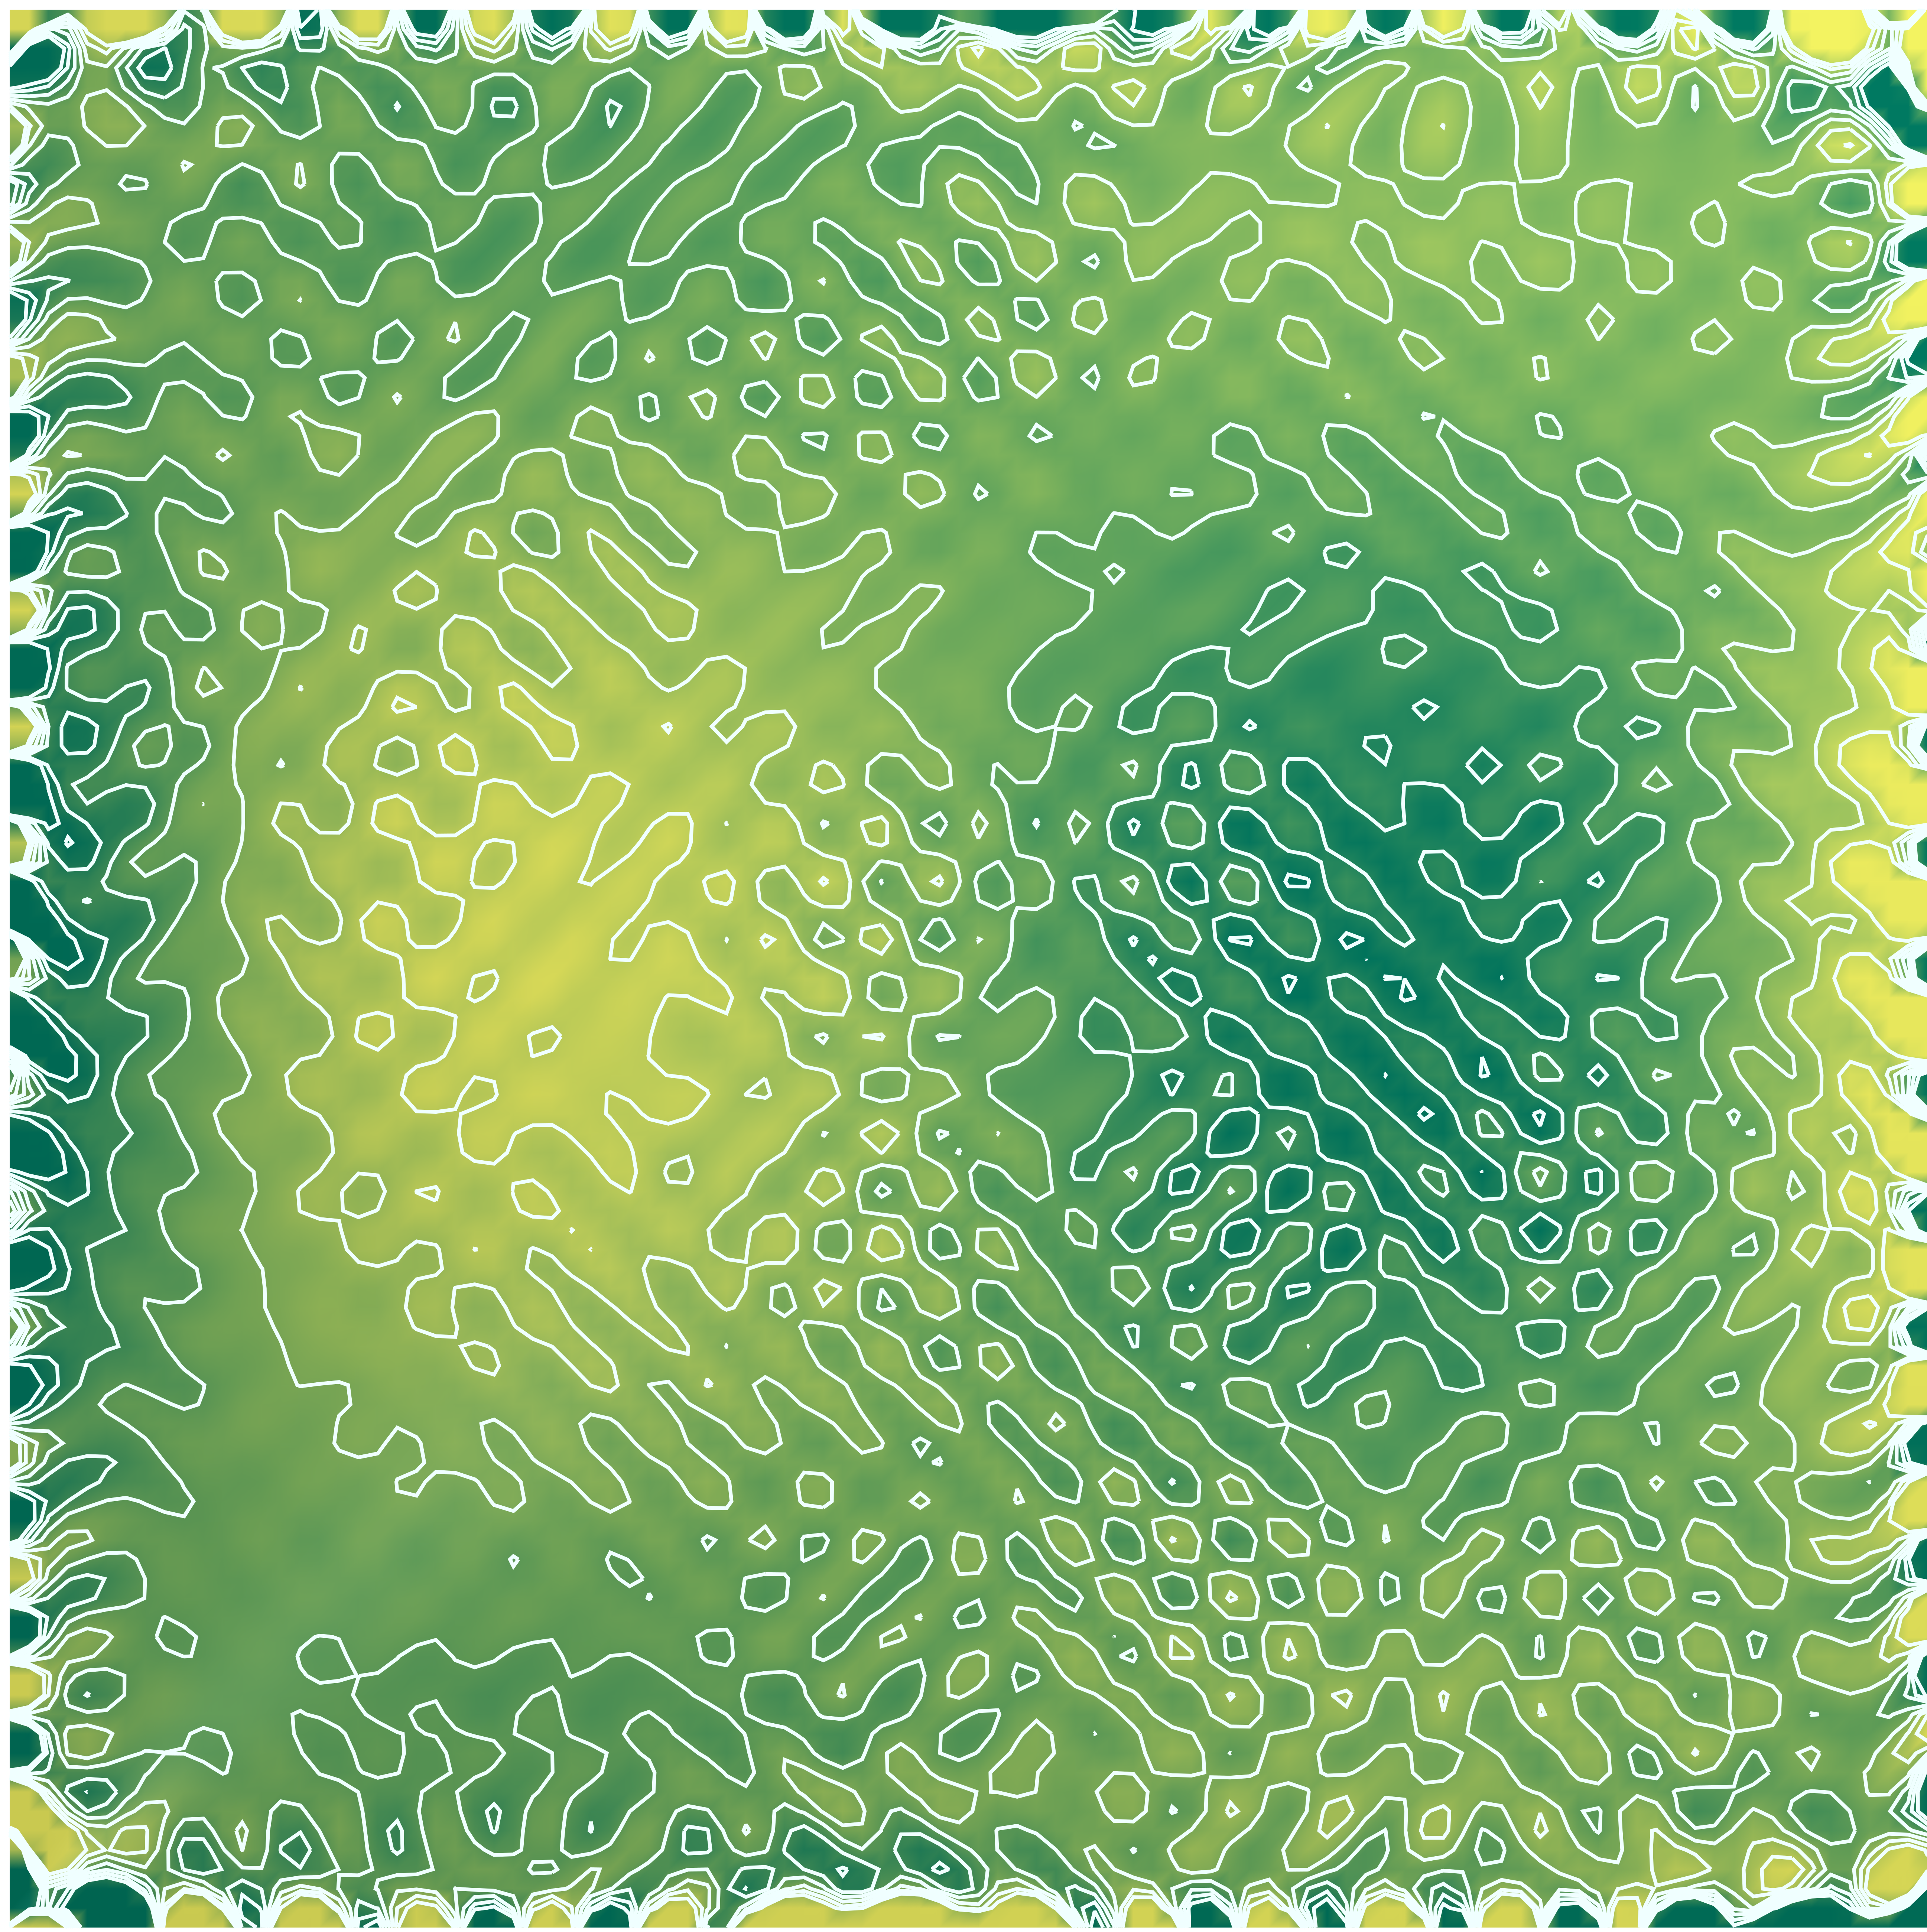
\includegraphics[width=0.45\textwidth]{figures/ch_5/SquarePlate_mix_tri6_q1_16_16.png}}
         & \raisebox{-0.7\height}{\includegraphics[width=0.45\textwidth]{figures/ch_5/SquarePlate_mix_tri6_q1_16_14.png}}& \\
         $n_p=1089$&$n_p=841$& \\
         \raisebox{-0.7\height}{\includegraphics[width=0.45\textwidth]{figures/ch_5/SquarePlate_mix_tri6_q1_16_12.png}}
        & & \\
        $n_p=625$& & \\
        \end{tabular}
    \end{subcaptiongroup}
    \caption{固支方板问题Tri6单元应力云图}\label{ch_5:fig:plate_tri6_q}
\end{figure}

\begin{figure}[!h]
    \centering
    \begin{subcaptiongroup}
        \begin{tabular}{c@{\hspace{0pt}}c}
          \raisebox{-0.8\height}{\includegraphics[width=0.5\textwidth]{figures/ch_5/SquarePlate_l2_u.png}}
        & \raisebox{-0.8\height}{\includegraphics[width=0.5\textwidth]{figures/ch_5/SquarePlate_l2_p.png}}\\
        \end{tabular}
    \end{subcaptiongroup}
    \caption{固支方板问题误差对比}\label{ch_5:fig:SquarePlate_l2}
\end{figure}

\clearpage
\subsection{Razzaque斜板问题}
考虑如图\ref{ch_5:fig:Razzaque_plate}所示斜板问题,其中斜板的边长为$L=100$,厚度为$h$,板内作用竖直向下的均布荷载作用$\bar{q}=1$,材料系数分别为杨氏模量$E=1085$、泊松比$\nu=0.31$。该斜板中心A点位移$\bar w_A$的参考解为:
\begin{equation} 
    \bar{w_A}=w_c\times10^2\frac{D}{\bar{q}L^4}
\end{equation}
\begin{figure}[!h]
    \centering 
        \includegraphics[scale=0.8]{figures/ch_5/skew_plate.png}
        \caption{Razzaque斜板问题模型}\label{ch_5:fig:Razzaque_plate}
\end{figure}

根据上文提出的固支方板混合离散方案,Razzaque斜板问题的混合离散方案如图\ref{ch_5:fig:Razzaque_plate_msh}所示。其约束自由度关系满足$n_q<\bar n_u$。
\begin{figure}[!h]
    \centering
        \begin{tabular}{c@{\hspace{24pt}}c}
            \includegraphics[width=0.40\textwidth]{figures/ch_5/SkewPlate_8_msh.png} &
            \includegraphics[width=0.40\textwidth]{figures/ch_5/SkewPlate_16_msh.png} \\
            $n_u=81$,$n_q=49$ & $n_u=289$,$n_q=225$ \\
            \includegraphics[width=0.40\textwidth]{figures/ch_5/SkewPlate_32_msh.png} &
            \includegraphics[width=0.40\textwidth]{figures/ch_5/SkewPlate_64_msh.png} \\
            $n_u=1089$,$n_q=961$ & $n_u=4225$,$n_q=3969$ \\
            \raisebox{-0.3\height}{\includegraphics[width=14pt]{figures/legend_u.png}} :挠度节点 &
            \raisebox{-0.3\height}{\includegraphics[width=14pt]{figures/legend_q.png}} :剪切应力节点 
        \end{tabular}
        \caption{有限元无网格混合离散方案}\label{ch_5:fig:Razzaque_plate_msh}
\end{figure}

图\ref{ch_5:fig:Razzaque_plate_q}和图\ref{ch_5:fig:Razzaque_plate_q2}为Razzaque斜板问题应力云图。从图中可以看出,无论是线性单元还是二次单元,传统混合离散方案都存在显著的应力振荡现象,而上述混合离散方案则有效的缓解了应力振荡现象。


\begin{figure}[!h]
    \centering
    \begin{subcaptiongroup}
        \begin{tabular}{c@{\hspace{0pt}}c@{\hspace{0pt}}c}
         传统混合离散方案&所提混合离散方案& \\
         \raisebox{-0.7\height}{\includegraphics[width=0.45\textwidth]{figures/ch_5/MorleysAcuteSkewPlate_tri3_q1_16_16.png}}
         & \raisebox{-0.7\height}{\includegraphics[width=0.45\textwidth]{figures/ch_5/MorleysAcuteSkewPlate_tri3_q1_16_12.png}}& \\
         Tri3单元 $n_p=81$&$n_p=49$&   \\
         \raisebox{-0.7\height}{\includegraphics[width=0.45\textwidth]{figures/ch_5/MorleysAcuteSkewPlate_quad4_q1_16_16.png}}
        & \raisebox{-0.7\height}{\includegraphics[width=0.45\textwidth]{figures/ch_5/MorleysAcuteSkewPlate_quad4_q1_16_12.png}}& \\
        Quad4单元 $n_p=289$&$n_p=225$&\\
        \end{tabular}
    \end{subcaptiongroup}
    \caption{Razzaque斜板问题线性单元应力云图}\label{ch_5:fig:Razzaque_plate_q}
\end{figure}

\begin{figure}[!h]
    \centering
    \begin{subcaptiongroup}
        \begin{tabular}{c@{\hspace{0pt}}c@{\hspace{0pt}}c}
         传统混合离散方案&所提混合离散方案& \\
         \raisebox{-0.7\height}{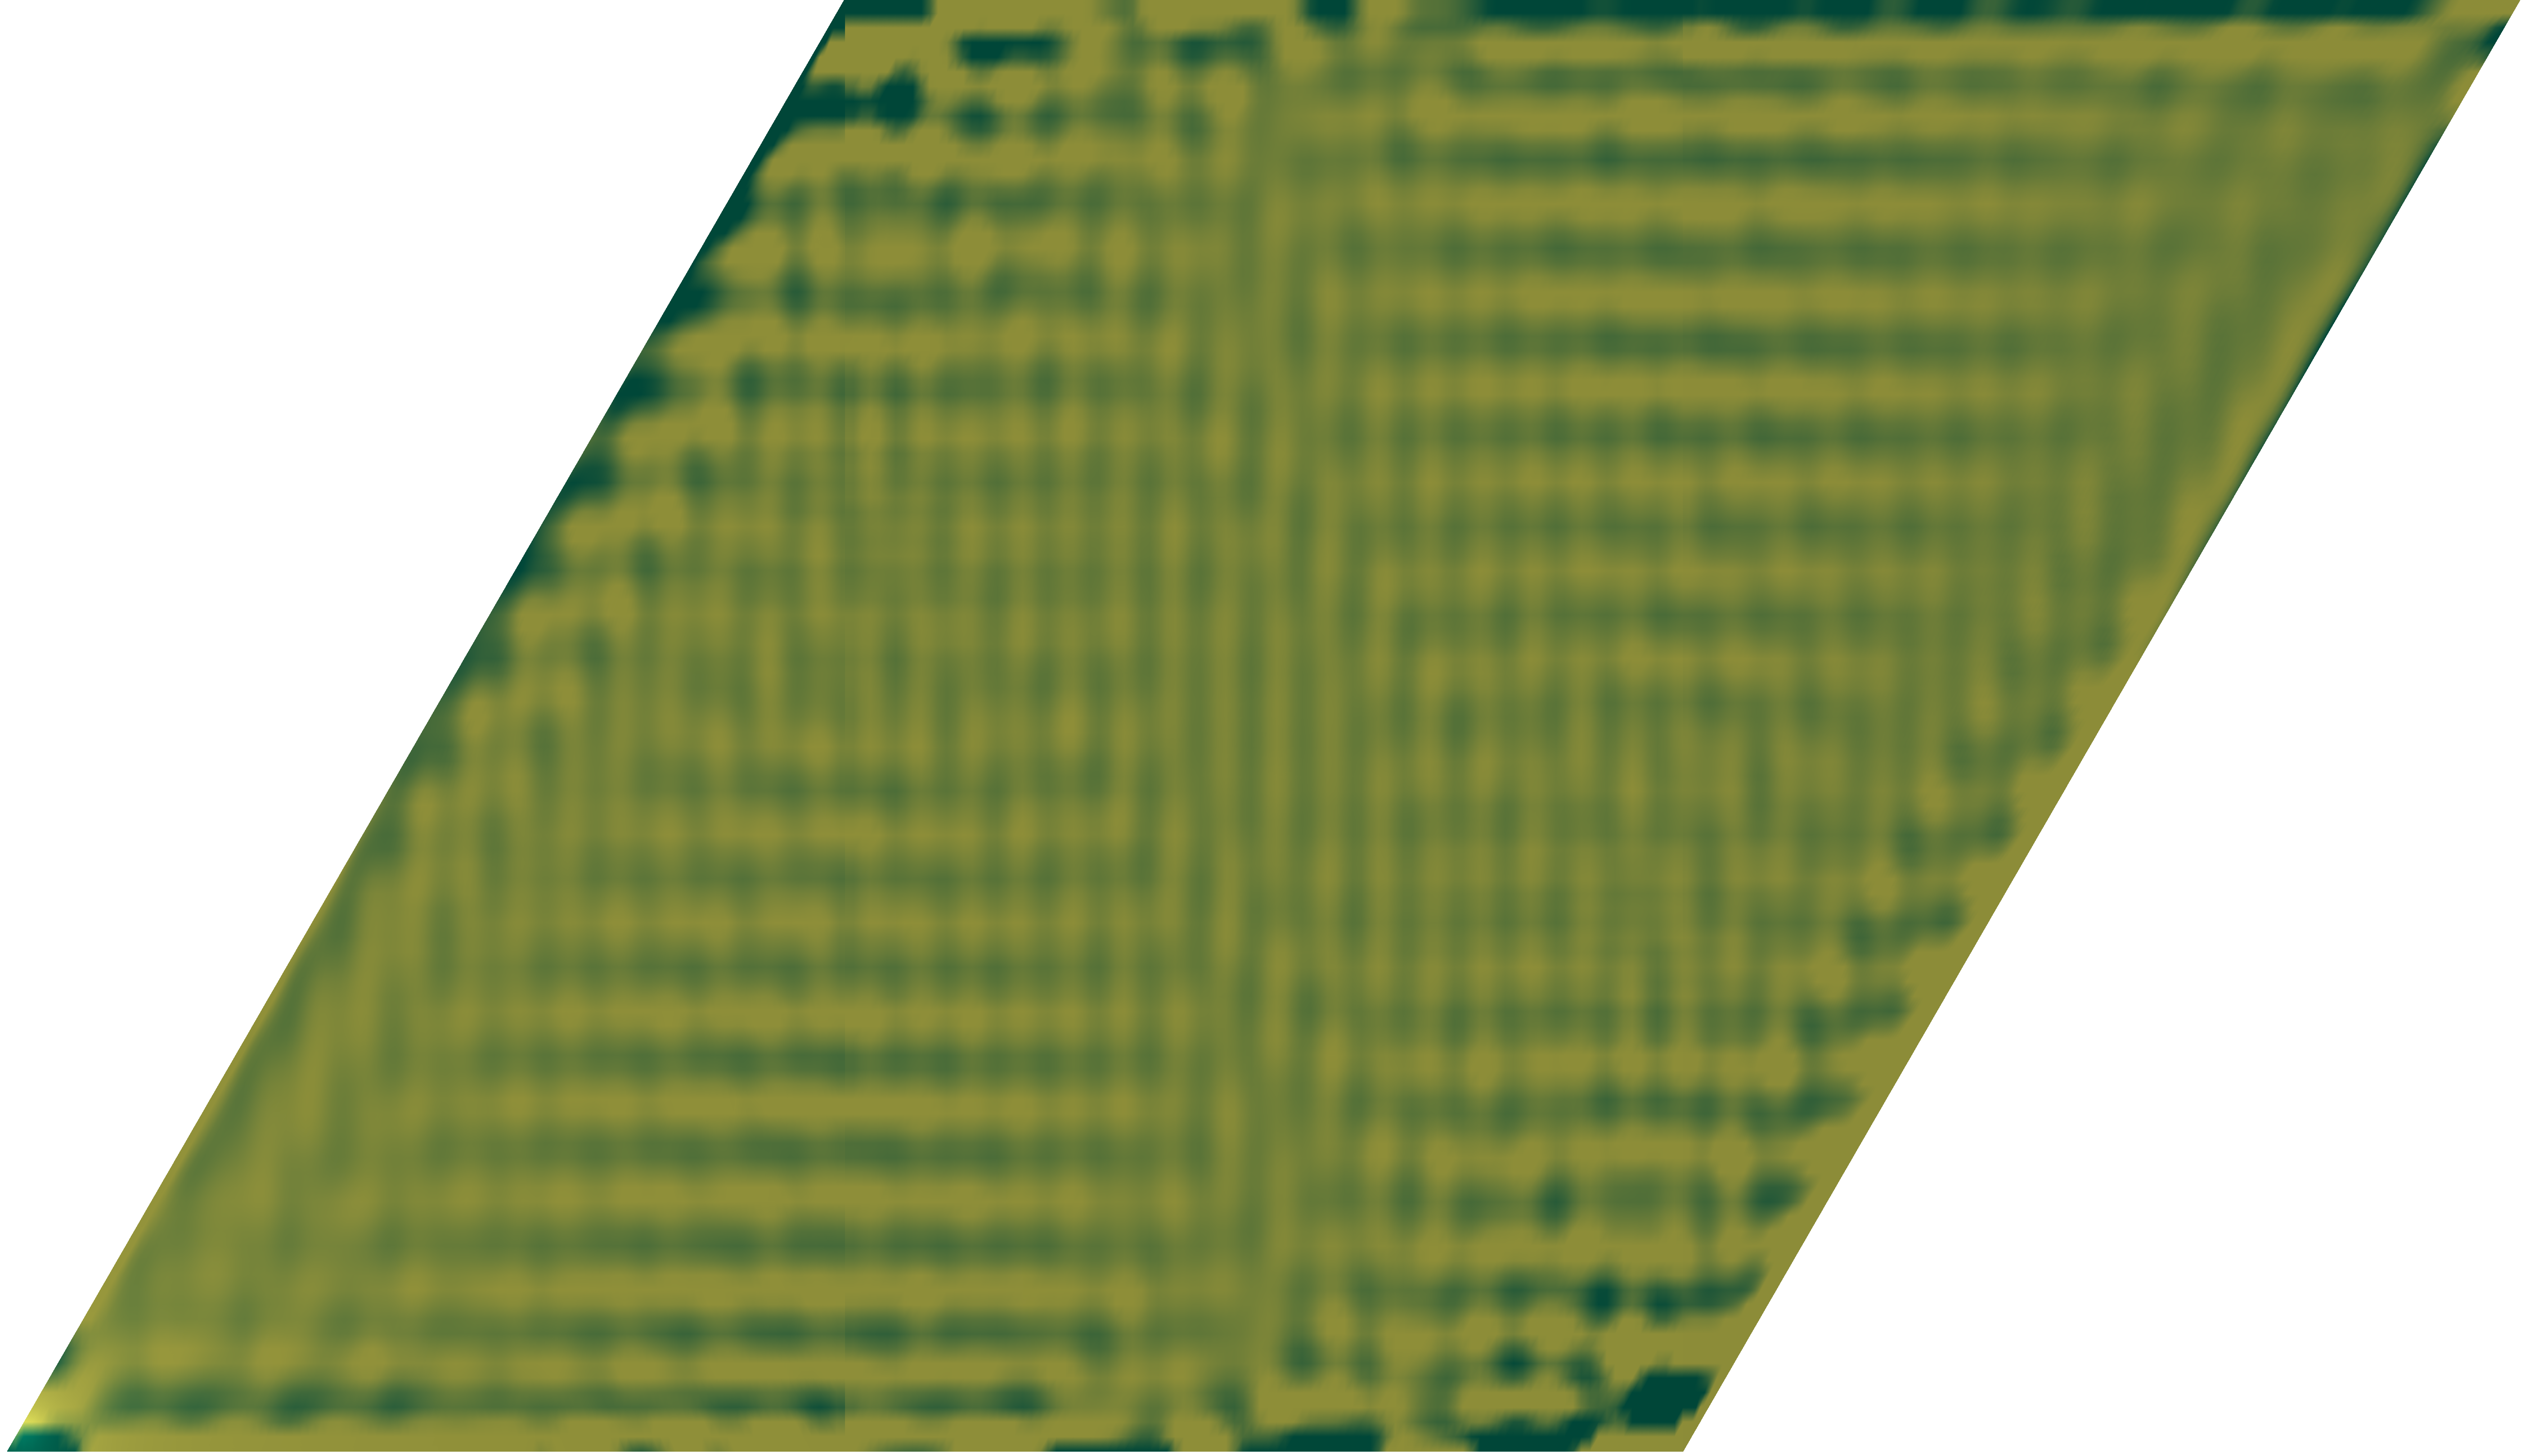
\includegraphics[width=0.45\textwidth]{figures/ch_5/MorleysAcuteSkewPlate_tri6_q1_16_16.png}}
         & \raisebox{-0.7\height}{\includegraphics[width=0.45\textwidth]{figures/ch_5/MorleysAcuteSkewPlate_tri6_q1_16_14.png}}& \\
         Tri6单元 $n_p=1089$&$n_p=841$&  \\
         \raisebox{-0.7\height}{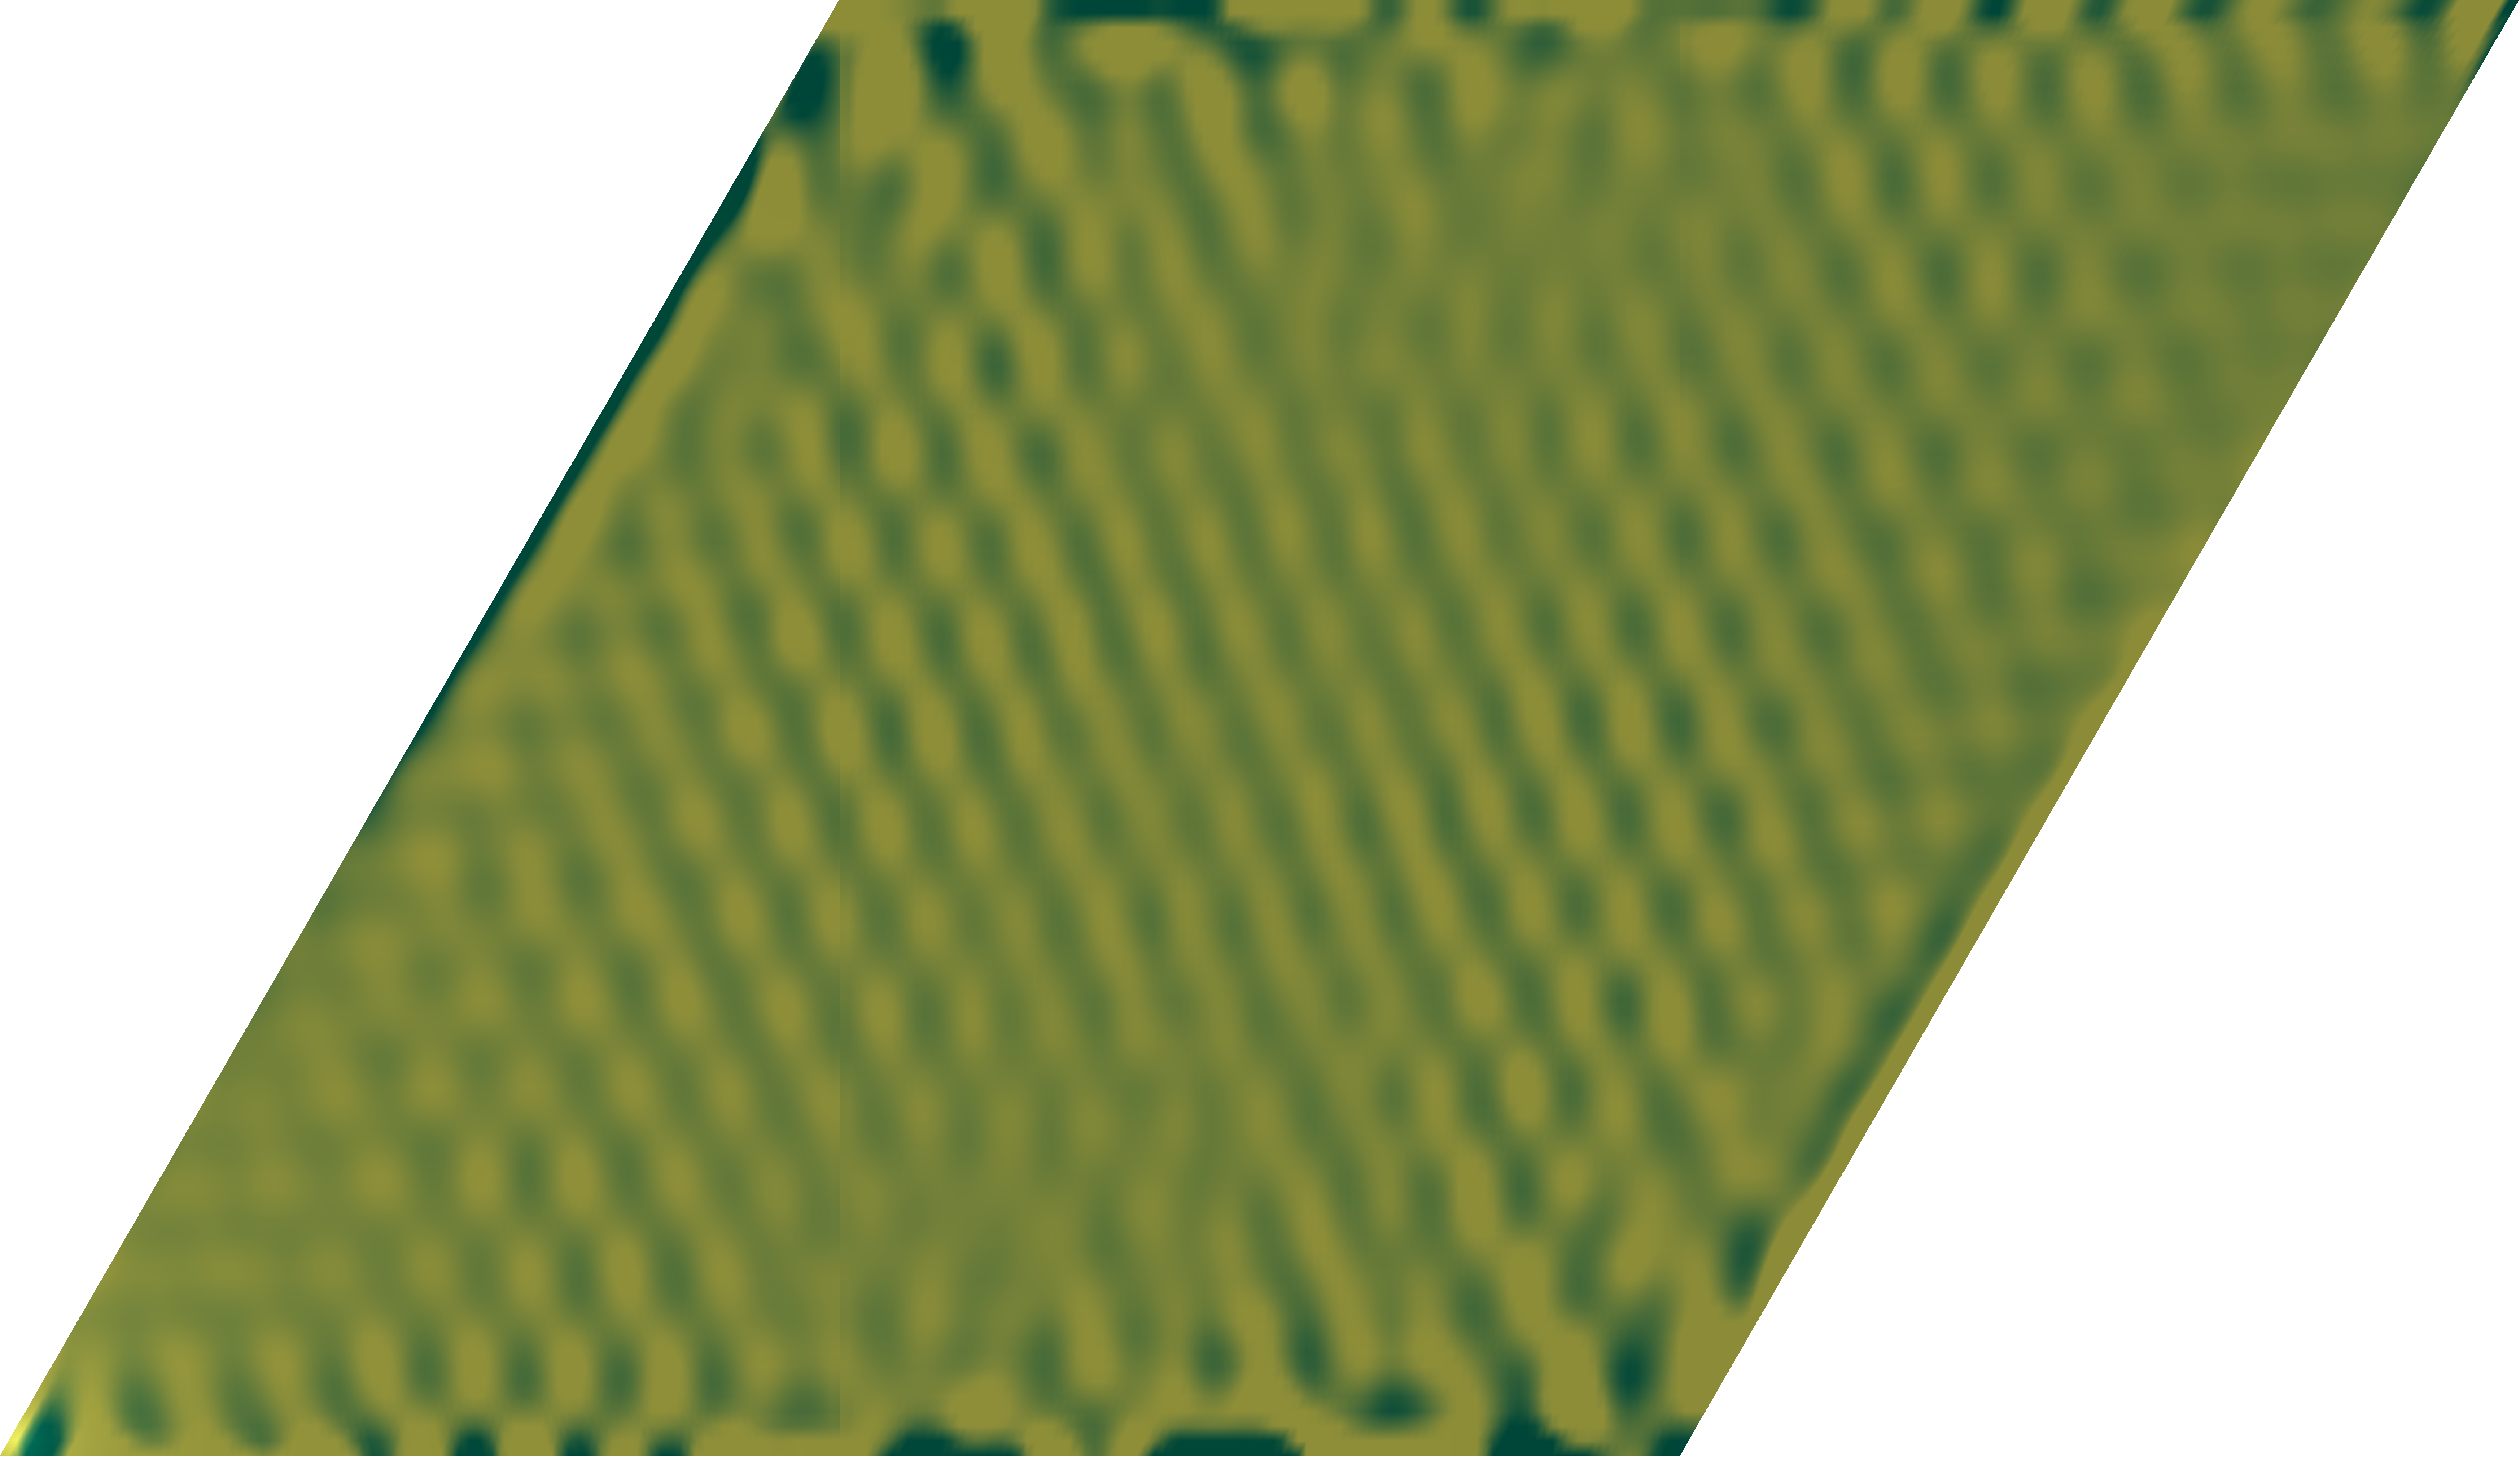
\includegraphics[width=0.45\textwidth]{figures/ch_5/MorleysAcuteSkewPlate_quad8_q1_16_16.png}}
        & \raisebox{-0.7\height}{\includegraphics[width=0.45\textwidth]{figures/ch_5/MorleysAcuteSkewPlate_quad8_q1_16_14.png}}& \\
        Quad8单元 $n_p=833$&$n_p=645$&\\
        \end{tabular}
    \end{subcaptiongroup}
    \caption{Razzaque斜板问题二次单元应力云图}\label{ch_5:fig:Razzaque_plate_q2}
\end{figure}


\clearpage
\subsection{简支圆板问题}
考虑如图\ref{ch_5:fig:Circular}所示简支圆板问题,其中圆板的半径为$R=5$,厚度为$h=0.1$,均匀荷载作用在板内为$\bar{q}=1$,材料系数分别为杨氏模量$E=10.92$、泊松比$\nu=0.3$。该圆板中心A点位移$w_A$的精确解为:$w_A=39831$。根据圆板的对称性,选取四分之一圆的域作为研究对象。

\begin{figure}[!h]
    \centering 
        \includegraphics[scale=0.8]{figures/ch_5/Circular.png}
        \caption{简支圆板问题模型}\label{ch_5:fig:Circular}
\end{figure}

简支圆板问题的混合离散方案如图\ref{ch_5:fig:Circular_msh}所示。其约束自由度关系满足$n_q<\bar n_u$。
\begin{figure}[!h]
    \centering
        \begin{tabular}{c@{\hspace{24pt}}c}
            \includegraphics[width=0.27\textwidth]{figures/ch_5/Circular_8_msh.png} &
            \includegraphics[width=0.27\textwidth]{figures/ch_5/Circular_16_msh.png} \\
            $n_u=61$,$n_q=37$ & $n_u=217$,$n_q=169$ \\
            \includegraphics[width=0.27\textwidth]{figures/ch_5/Circular_32_msh.png} &
            \includegraphics[width=0.27\textwidth]{figures/ch_5/Circular_64_msh.png} \\
            $n_u=817$,$n_q=721$ & $n_u=3169$,$n_q=2977$ \\
            \raisebox{-0.3\height}{\includegraphics[width=14pt]{figures/legend_u.png}} :挠度节点 &
            \raisebox{-0.3\height}{\includegraphics[width=14pt]{figures/legend_q.png}} :剪切应力节点 
        \end{tabular}
        \caption{有限元无网格混合离散方案}\label{ch_5:fig:Circular_msh}
\end{figure}

图\ref{ch_5:fig:Circular_q}和图\ref{ch_5:fig:Circular_q2}为简支圆板问题应力云图。从图中可以看出,无论是线性单元还是二次单元,传统混合离散方案都存在显著的应力振荡现象,而上述混合离散方案则有效的缓解了应力振荡现象。


\begin{figure}[!h]
    \centering
    \begin{subcaptiongroup}
        \begin{tabular}{c@{\hspace{0pt}}c@{\hspace{0pt}}c}
         传统混合离散方案&所提混合离散方案& \\
         \raisebox{-0.5\height}{\includegraphics[width=0.45\textwidth]{figures/ch_5/Circular_tri3_q1_32_32.png}}
         & \raisebox{-0.5\height}{\includegraphics[width=0.45\textwidth]{figures/ch_5/Circular_tri3_q1_32_26.png}}& \\
         Tri3单元 $n_p=817$&$n_p=721$&   \\
         \raisebox{-0.5\height}{\includegraphics[width=0.45\textwidth]{figures/ch_5/Circular_quad4_q1_32_32.png}}
        & \raisebox{-0.5\height}{\includegraphics[width=0.45\textwidth]{figures/ch_5/Circular_quad4_q1_32_26.png}}& \\
        Quad4单元 $n_p=817$&$n_p=721$&\\
        \end{tabular}
    \end{subcaptiongroup}
    \caption{简支圆板问题线性单元应力云图}\label{ch_5:fig:Circular_q}
\end{figure}

\clearpage
\begin{figure}[!h]
    \centering
    \begin{subcaptiongroup}
        \begin{tabular}{c@{\hspace{0pt}}c@{\hspace{0pt}}c}
         传统混合离散方案&所提混合离散方案& \\
         \raisebox{-0.5\height}{\includegraphics[width=0.45\textwidth]{figures/ch_5/Circular_tri6_q1_16_16.png}}
         & \raisebox{-0.5\height}{\includegraphics[width=0.45\textwidth]{figures/ch_5/Circular_tri6_q1_16_12.png}}& \\
         Tri6单元 $n_p=817$&$n_p=631$&   \\
         \raisebox{-0.5\height}{\includegraphics[width=0.45\textwidth]{figures/ch_5/Circular_quad8_q1_16_16.png}}
        & \raisebox{-0.5\height}{\includegraphics[width=0.45\textwidth]{figures/ch_5/Circular_quad8_q1_16_12.png}}& \\
        Quad8单元 $n_p=625$&$n_p=484$&\\
        \end{tabular}
    \end{subcaptiongroup}
    \caption{简支圆板问二次单元应力云图}\label{ch_5:fig:Circular_q2}
\end{figure}

\section{小结}
本章深入探讨了基于LBB稳定性条件的有限元无网格混合离散方案在剪切自锁问题中的应用。
首先,从中厚板问题的本构特性出发,系统分析了传统有限元法在数值求解中厚板问题时产生剪切自锁问题的根本原因。
随后,结合混合离散公式与再生核无网格近似理论,提出了适用于中厚板问题的有限元无网格混合离散分析方法。基于考虑约束比的LBB稳定系数估计以及中厚板问题的多项式空间,确定了中厚板问题的最优约束比取值范围。
最后,通过对经典中厚板算例的数值分析,提出了能够缓解中厚板剪切自锁的有限元无网格混合离散方案。数值结果表明,与传统混合离散方案相比,本文所提出的混合离散方案能够显著缓解应力振荡现象,进一步验证了LBB稳定系数估计出的最优约束比范围的正确性以及所提混合离散方案在数值稳定方面的优越性。